\documentclass[11pt]{article}

\usepackage[a4paper, total={6in, 9in}]{geometry}
\usepackage{graphicx}
\usepackage{tabularx}
\usepackage{float}
\usepackage{amsmath}
\usepackage{hyperref}
\usepackage{fancyhdr}
\usepackage{lastpage}

\def\greedyeps{0}
\def\greedyalph{0.9}
\def\scheduleeps{0}
\def\schedulealph{0.55}
\def\sarsaalph{0.55}

\title{\vspace{-3cm}Reinforcement Learning TP3 report}
\author{Juliette Jacquot, Matis Braun}
\date{}

\begin{document}

\maketitle

\pagestyle{fancy}
\renewcommand\headrulewidth{1pt}
\renewcommand\footrulewidth{1pt}
\setlength{\headheight}{14pt}
\fancyhead[L]{Reinforcement Learning report}
\fancyhead[R]{Juliette Jacquot, Matis Braun}
\fancyfoot[C]{Page \thepage/\pageref*{LastPage}}

\section*{Introduction}

In this report, we teach some reinforcement learning models to play to the game "Taxi-v3" from OpenAI Gym.

This game contains a 5 by 5 grid, a taxi a passenger, and a building.
The taxi can move in four directions (up, down, left, right), pick up a passenger on its current spot, or drop a passenger off on its current spot.
The goal of the game is to pick up the passenger and bring them to the building as fast as possible.

Each model is trained over a thousand iterations of the game, and is allowed to choose up to 200 actions to execute in the span of a game.

\section*{Models}

\subsection*{QLearning}

%We first use some models based on the QLearning algorithm.
%More specifically, we study the results of its $\varepsilon$-greedy and $\varepsilon$ scheduling variants,
%which can influence the exploration of possibilities during the model's training with the parameter $\varepsilon$.

\subsubsection*{$\varepsilon$-greedy}

%We first tested the QLearning algorithm on dummy parameters ($\varepsilon = 0.25$, $\alpha=0.5$, $\gamma=0.99$), before doing a hyperparameter search for $\varepsilon$ and the learning rate $\alpha$.

Surprisingly, as seen in figure \ref{fig:qlearning_eps_search}, trying to add exploration to the QLearning algorithm is detrimental to the model's performance.
Perhaps the size of the game environment and the constant negative rewards applied until the end of the game prevent the model from finding a local maximum reward, making the added exploration unnecessary.

On the other hand, the learning rate does not seem to have much of an influence on the final result, as seen in figure \ref{fig:qlearning_alph_search}.
Indeed, the final reward seems to stabilize around a singular value as soon as $\alpha \geq 0.2$.

As seen in figures \ref{fig:qlearning_base_reward} and \ref{fig:qlearning_opti_reward}, setting the parameter $\varepsilon$ at \greedyeps\ stabilizes the rewards almost immediately once the model has an idea of how to play the game.

\subsubsection*{$\varepsilon$ scheduling}

In the $\varepsilon$ scheduling version of the QLearning algorithm, the chance of a random choice occurring in the model decreases as time goes on.
Still, as seen in figure \ref{fig:qlearning_eps_schedule_eps_search}, the model gets better results when no random choice occurs at all.
Similarly, the learning rate behaves the same way as in the $\varepsilon$-greedy variant of the model, as seen in figure \ref{fig:qlearning_eps_schedule_alph_search}.
While the difference in stability between the model with dummy parameters (figure \ref{fig:qlearning_esp_schedule_base_reward}) and the one with optimized parameters (figure \ref{fig:qlearning_eps_schedule_opti_reward}) is reduced, there is still a noticeable improvement when $\varepsilon = \scheduleeps$.

\subsection*{SARSA}

Unlike the QLearning algorithm, SARSA does not use a random chance to explore.
However, figure \ref{fig:sarsa_alph_search} shows the same stabilization of rewards depending on $\alpha$ than the other algorithms.
As such, there is not an easily perceived difference between the base model (figure \ref{fig:sarsa_base_reward}) and the optimized one (figure \ref{fig:sarsa_optimized_reward}).

\section*{Conclusion}

The optimized versions of each algorithm seem to behave similarly, both in their learning and in their final results as seen in figure \ref{fig:final_rewards}.

\newpage

\fancyfoot[L]{Appendix}

\section*{Appendix}

\vspace{-1.5em}
\rule{\textwidth}{0.5pt}

\vspace{1em}

\begin{figure}[H]
	\centering
	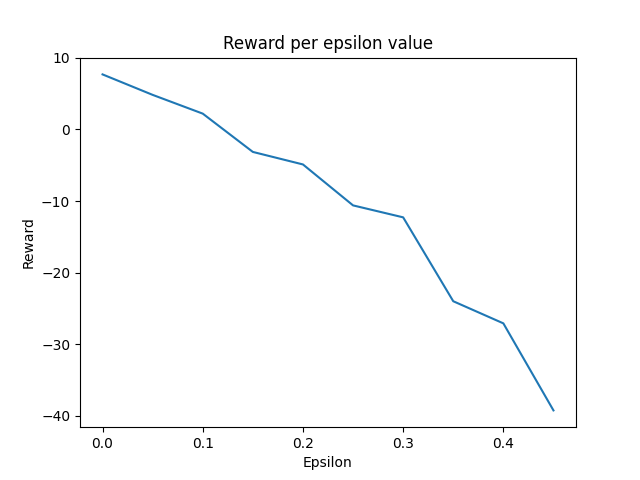
\includegraphics[width=12cm]{../figures/part_1/learning_reward_qlearning_eps_search.png}
	\caption{Average final rewards for QLearning per $\varepsilon$ ($\alpha = 0.5$)}
	\label{fig:qlearning_eps_search}
\end{figure}

\begin{figure}[H]
	\centering
	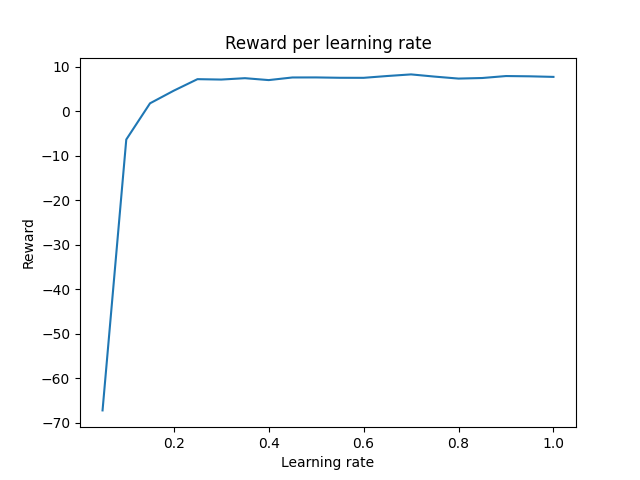
\includegraphics[width=12cm]{../figures/part_1/learning_reward_qlearning_alpha_search.png}
	\caption{Average final rewards for QLearning per $\alpha$ ($\varepsilon = \greedyeps$)}
	\label{fig:qlearning_alph_search}
\end{figure}

\begin{figure}[H]
	\centering
	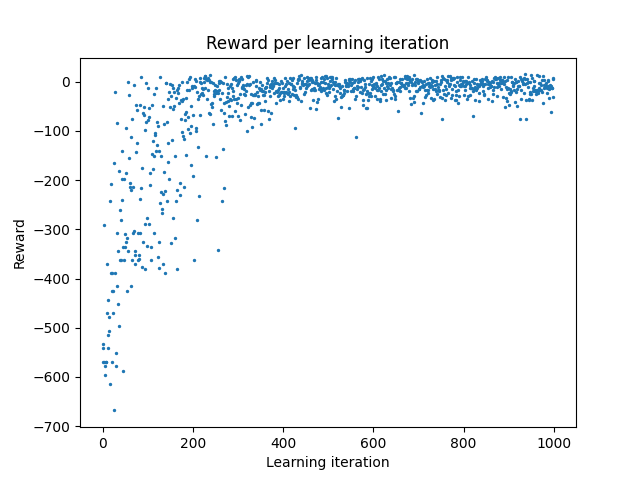
\includegraphics[width=12cm]{../figures/part_1/learning_reward_base_qlearning.png}
	\caption{QLearning rewards during learning process ($\alpha = 0.5$, $\varepsilon = 0.25$)}
	\label{fig:qlearning_base_reward}
\end{figure}

\begin{figure}[H]
	\centering
	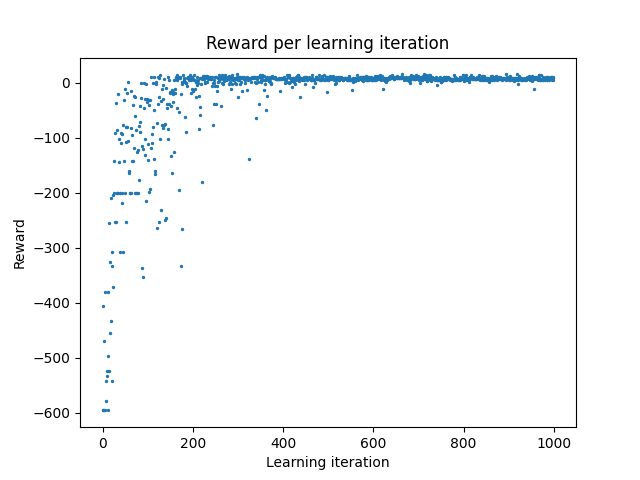
\includegraphics[width=12cm]{../figures/part_1/learning_reward_optimized_qlearning.png}
	\caption{QLearning rewards during learning process ($\alpha = \greedyalph$, $\varepsilon = \greedyeps$)}
	\label{fig:qlearning_opti_reward}
\end{figure}

\begin{figure}[H]
	\centering
	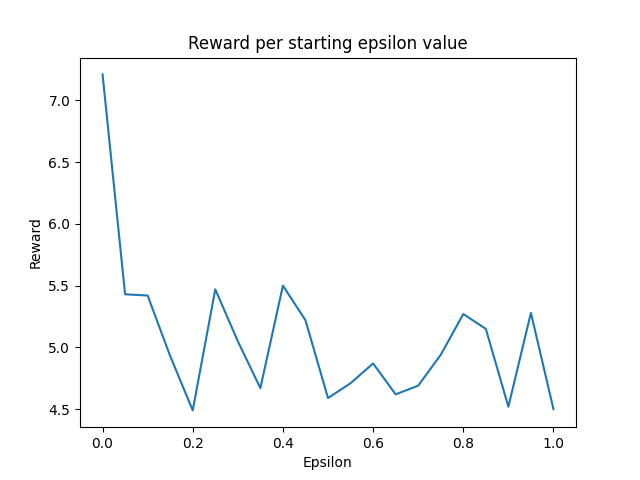
\includegraphics[width=12cm]{../figures/part_2/learning_reward_qlearning_eps_schedule_start_eps_search.png}
	\caption{Average final rewards for QLearning with $\varepsilon$ scheduling per $\varepsilon_{\text{start}}$\\($\alpha = 0.5$)}
	\label{fig:qlearning_eps_schedule_eps_search}
\end{figure}

\begin{figure}[H]
	\centering
	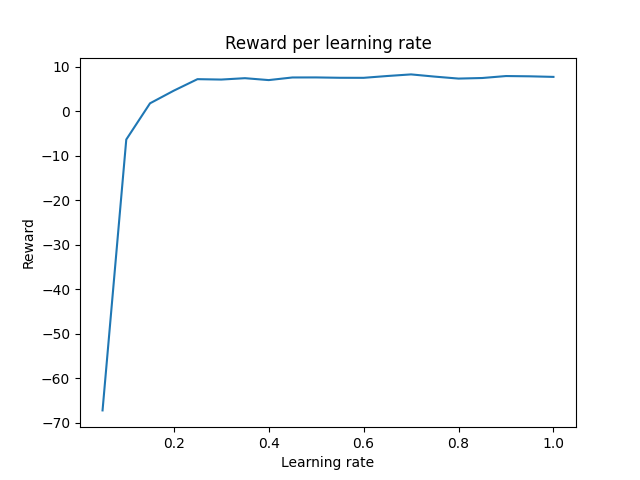
\includegraphics[width=12cm]{../figures/part_1/learning_reward_qlearning_alpha_search.png}
	\caption{Average final rewards for QLearning with $\varepsilon$ scheduling per $\alpha$\\($\varepsilon = \scheduleeps$)}
	\label{fig:qlearning_eps_schedule_alph_search}
\end{figure}

\begin{figure}[H]
	\centering
	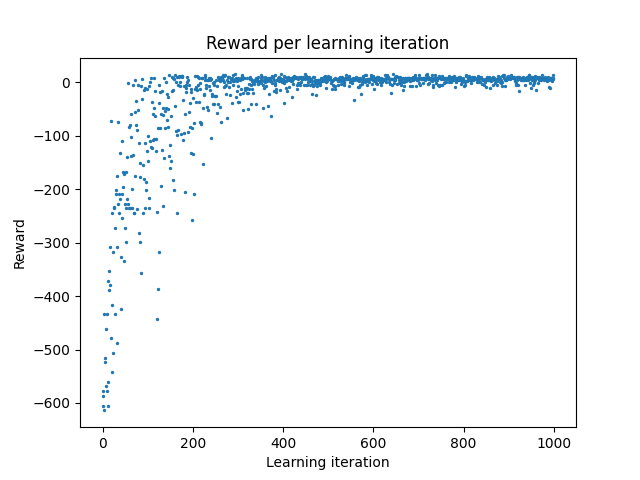
\includegraphics[width=12cm]{../figures/part_2/learning_reward_base_qlearning_eps_schedule.png}
	\caption{QLearning with $\varepsilon$ scheduling rewards during learning process\\($\alpha = 0.5$, $\varepsilon_{\text{start}} = 0.25$)}
	\label{fig:qlearning_esp_schedule_base_reward}
\end{figure}

\begin{figure}[H]
	\centering
	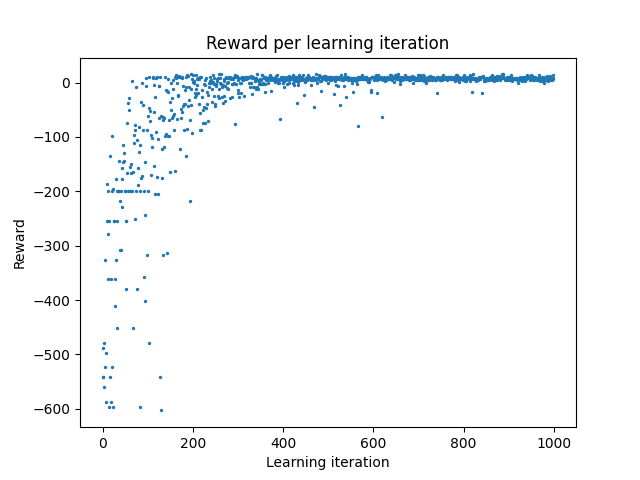
\includegraphics[width=12cm]{../figures/part_2/learning_reward_optimized_qlearning_eps_schedule.png}
	\caption{QLearning with $\varepsilon$ scheduling rewards during learning process\\($\alpha = \schedulealph$, $\varepsilon_{\text{start}} = \scheduleeps$)}
	\label{fig:qlearning_eps_schedule_opti_reward}
\end{figure}

\begin{figure}[H]
	\centering
	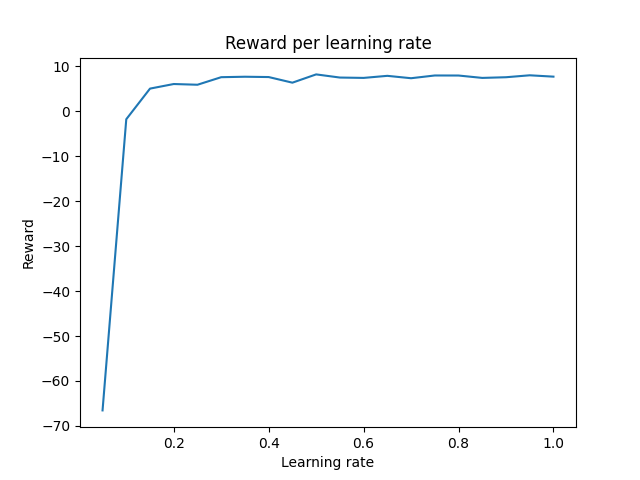
\includegraphics[width=12cm]{../figures/part_3/learning_reward_sarsa_alpha_search.png}
	\caption{Average final rewards for Sarsa per $\alpha$}
	\label{fig:sarsa_alph_search}
\end{figure}

\begin{figure}[H]
	\centering
	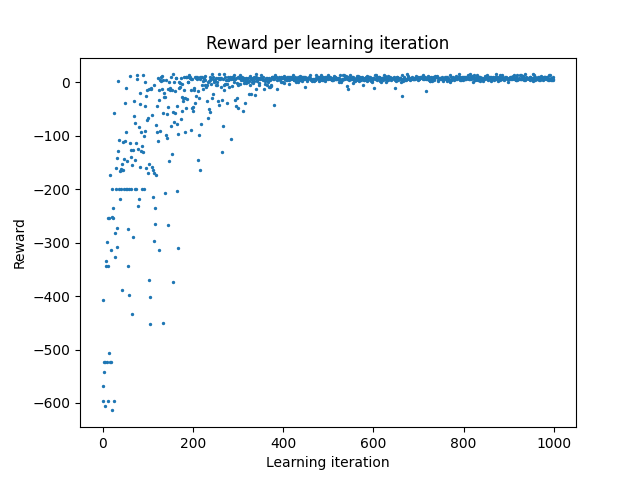
\includegraphics[width=12cm]{../figures/part_3/learning_reward_base_sarsa.png}
	\caption{Sarsa rewards during learning process ($\alpha = 0.5$)}
	\label{fig:sarsa_base_reward}
\end{figure}

\begin{figure}[H]
	\centering
	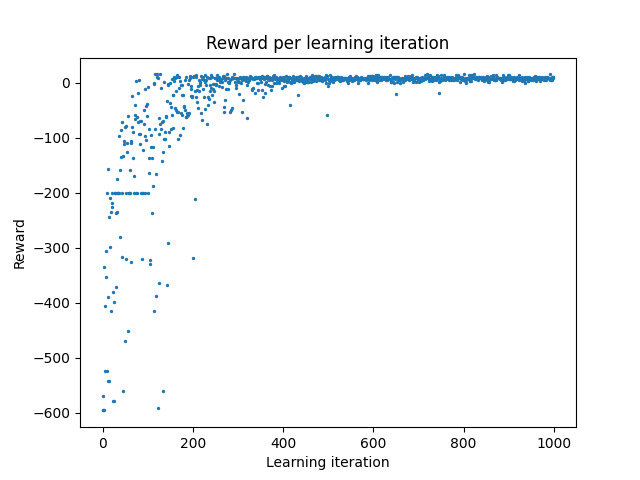
\includegraphics[width=12cm]{../figures/part_3/learning_reward_optimized_sarsa.png}
	\caption{Sarsa rewards during learning process ($\alpha = \sarsaalph$)}
	\label{fig:sarsa_optimized_reward}
\end{figure}

\begin{figure}[H]
	\centering
	\begin{tabular}{c | c | c | c}
		& $\varepsilon$-greedy QLearning	& QLearning with $\varepsilon$ scheduling	& Sarsa \\
		\hline
		Reward	& 7.78 & 7.69 & 7.49
	\end{tabular}
	\caption{Final rewards for all models}
	\label{fig:final_rewards}
\end{figure}

\end{document}